% Source: http://www.brian-amberg.de/uni/poster/
\documentclass[landscape,archE,fontscale=0.2]{baposter}
\usepackage[vlined]{algorithm2e}
\usepackage{times,calc}
\usepackage{amsmath,amssymb}
\usepackage{relsize}
\usepackage{multirow,multicol}
\usepackage{ae}
\usepackage{url}

\usepackage[T1]{fontenc}
\renewcommand{\familydefault}{\sfdefault}

\usepackage{enumitem}\setlist{nolistsep,leftmargin=*}
\usepackage{graphicx}\graphicspath{{images/}}

\usepackage{tikz}
\usetikzlibrary[topaths]
\newcount\mycount

\usepackage[
citestyle=numeric,
firstinits=true,
maxcitenames=1,
]{biblatex}
\bibliography{refs}

\setlength{\columnsep}{0.7em}\setlength{\columnseprule}{0mm}

\definecolor{crimsonRed}{cmyk}{0, 1, 1, 0.4}

\begin{document}
\begin{poster}{
    grid=false,
    colspacing=0.7em,
    headerColorOne=crimsonRed, borderColor=crimsonRed,
    textborder=faded,
    headerborder=open, headershape=roundedright,
    headershade=plain, headerFontColor=white,
    background=none, bgColorOne=white,
    headerheight=0.15\textheight,
    headerfont=\color{white}\textsf\textbf\Large,
    columns=3
  }{
    \includegraphics[height=0.13\textheight]{cmu-seal}
  }{
    {\textsc{\textbf{\LARGE Title}}} \\
    {\Large Subtitle}
  }{\vspace{2mm}\large
    Brandon Amos and $\ldots$ \\
    School of Computer Science,
    Carnegie Mellon University
  }{
    \includegraphics[height=0.11\textheight]{cmu-logo}
  }

  \headerbox{Introduction and Background}
  {name=intro,column=0,row=0}{\begin{itemize}
\item Item 1\cite{article}
\item Item 2
\item Item 3
\end{itemize}}

  \headerbox{Design}
  {name=design,column=1,row=0}{\begin{center}
  % http://www.texample.net/tikz/examples/complete-graph/
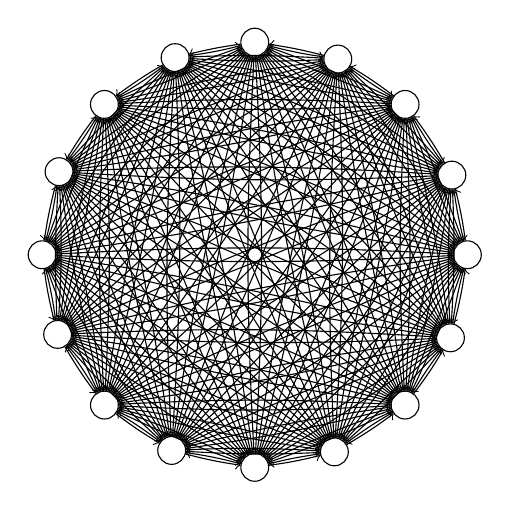
\begin{tikzpicture}[transform shape, scale=0.5]
  %the multiplication with floats is not possible. Thus I split the loop in two.
  \foreach \number in {1,...,8}{
      % Computer angle:
        \mycount=\number
        \advance\mycount by -1
  \multiply\mycount by 45
        \advance\mycount by 0
      \node[draw,circle,inner sep=0.25cm] (N-\number) at (\the\mycount:5.4cm) {};
    }
  \foreach \number in {9,...,16}{
      % Computer angle:
        \mycount=\number
        \advance\mycount by -1
  \multiply\mycount by 45
        \advance\mycount by 22.5
      \node[draw,circle,inner sep=0.25cm] (N-\number) at (\the\mycount:5.4cm) {};
    }
  \foreach \number in {1,...,15}{
        \mycount=\number
        \advance\mycount by 1
  \foreach \numbera in {\the\mycount,...,16}{
    \path (N-\number) edge[->,bend right=3] (N-\numbera)  edge[<-,bend
      left=3] (N-\numbera);
  }
}
\end{tikzpicture}
  % http://www.texample.net/tikz/examples/complete-graph/
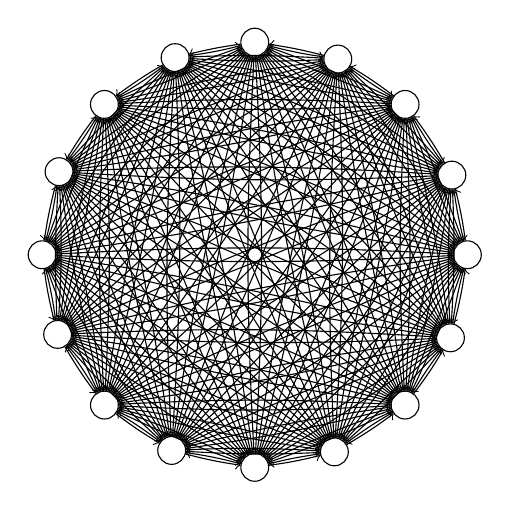
\begin{tikzpicture}[transform shape, scale=0.5]
  %the multiplication with floats is not possible. Thus I split the loop in two.
  \foreach \number in {1,...,8}{
      % Computer angle:
        \mycount=\number
        \advance\mycount by -1
  \multiply\mycount by 45
        \advance\mycount by 0
      \node[draw,circle,inner sep=0.25cm] (N-\number) at (\the\mycount:5.4cm) {};
    }
  \foreach \number in {9,...,16}{
      % Computer angle:
        \mycount=\number
        \advance\mycount by -1
  \multiply\mycount by 45
        \advance\mycount by 22.5
      \node[draw,circle,inner sep=0.25cm] (N-\number) at (\the\mycount:5.4cm) {};
    }
  \foreach \number in {1,...,15}{
        \mycount=\number
        \advance\mycount by 1
  \foreach \numbera in {\the\mycount,...,16}{
    \path (N-\number) edge[->,bend right=3] (N-\numbera)  edge[<-,bend
      left=3] (N-\numbera);
  }
}
\end{tikzpicture}
\end{center}}

  \headerbox{Results}
  {name=results,column=2}{\section{Empirical Evaluation of Learning}
\label{results}

\subsection{Experimental Platform}

In 2-3 paragraphs describe the experimental
platform that you used. For example, describe
the processor, memory, etc. that were in the
machine you used for experiments. List the OS
version, etc.

\subsection{Experiment 1: Pithy title of experiment}
\label{experiment1}

Give a 1-paragraph overview of the point of the experiment.
What were you trying to prove with the experiment? Make
sure and explain how the experiment fits into your overall
theme. Ideally, you will refer back to a challenge.

\textbf{Hypothesis: Pithy hypothesis heading.} Our
hypothesis was XYZ. Describe what you expected to
happen.

\textbf{Experiment 1 Results.} Include one or more
graphs, tables, or figures showing some hard data
from your experiments. Describe what is seen in the
graphs. Be very detailed in your discussions and make
sure that you label all aspects of your tables, figures,
graphs.

\subsection{Experiment 2: Pithy title of experiment}
\label{experiment2}

Give a 1-paragraph overview of the point of the experiment.
What were you trying to prove with the experiment? Make
sure and explain how the experiment fits into your overall
theme. Ideally, you will refer back to a challenge.

\textbf{Hypothesis: Pithy hypothesis heading.} Our
hypothesis was XYZ. Describe what you expected to
happen.

\textbf{Experiment 2 Results.} Include one or more
graphs, tables, or figures showing some hard data
from your experiments. Describe what is seen in the
graphs. Be very detailed in your discussions and make
sure that you label all aspects of your tables, figures,
graphs.

\subsection{Analysis of Results}
\label{analysis}

Describe what you learned from the empirical data
collected from the experiemnts. Why is the data
important? How does it show you did a good job
solving the problem? Does it prove that you are
better than existing approaches? Are there areas
where you do not perform as well? Describe
these things here.
}

  % Below lowest section.
  \headerbox{References}
  {name=refs,column=0,below=design,above=bottom,span=3}{
    \setlength{\bibitemsep}{0pt}
    \renewcommand*{\bibfont}{\footnotesize}
    \printbibliography[heading=none]
  }

  % Sections bordering references that aren't the lowest.
  \headerbox{Contributions}
  {name=contrib,column=0,below=intro,above=refs}{\input{contrib}}

  \headerbox{Conclusions}
  {name=conclusions,column=2,below=results,above=refs}{\begin{itemize}
\item Item 1
\item Item 2
\item Item 3
\item Item 4
\end{itemize}}

\end{poster}
\end{document}
